\section{Experiment Setup}
\label{sec:experimentSetup}
After developing the prototypes, we implemented a version of the hands from Job Simulator which we used as a baseline for comparison during our user evaluation. For the evaluation we decided to compare only one of the prototypes with the Job Simulator Hand, which was the Physics Hand.

During the evaluations, subjects tested our implementation of the Job Simulator Hand and our Physics Hand in two different environments and gave individual feedback. Each person would first play through what we call the Dev World environment, starting with the Job Simulator Hand to establish the baseline and then with the Physics Hand, after which they would do the same with a more game-like environment, which we call Touchy Island. The Dev World is a small-scale environment with a few basic objects that the users can interact with in different ways. Touchy Island is like a playground, where the player can interact with different creatures and objects on a floating island. The details of both these environments are noted below in Sections \ref{subsec:devWorld} and \ref{subsec:touchyIsland}. While experiencing the two hands in the Dev World, the users were prompted to follow a set of instructions, seen in Figure \ref{fig:listActionsDevWorld}, which would guide them through the different interactions possible with the hands to make sure they noticed their features. Besides these interactions, the instructions also mentioned the controls like using the trigger to close the hand. In order for the players to be able to move around the environments, which are larger than the play space of the HTC Vive, we made use of a Unity plugin called Vive-Teleporter \parencite{Biagioli2016}, which was slightly modified to solve problems with grabbing. Teleportation is activated using the trackpad on the controller.

\begin{figure}[h]
\begin{itemize}[noitemsep]
\item Press the triggers to close the hands.
\item Touch immovable object.
\item Move controller deep into immovable object to see real hand visualization.
\item Hover over a grabbable object.
\item Grab a grabbable object.
\item Move around the grabbed object.
\item Hit an object with a grabbed object.
\item Throw a grabbed object.
\item Push a movable object.
\item Break the joint set up between two of the grabbables by grabbing one of the objects with each hand and pulling in opposite directions.
\item Lift a grabbable object without grabbing it with the triggers.
\item Teleport using the trackpad on the controller.
\end{itemize}
\caption{List of actions the testers were guided through, while in the Dev World environment.}
\label{fig:listActionsDevWorld}
\end{figure}

When the testers had gone through the instructions in the Dev World for both hands, we continued to Touchy Island. In Touchy Island we would not guide them with specific instructions, but allow them to freely move around and experience the interactions possible. Sometimes we would hint at certain interactions or features of Touchy Island, if the testers hadn't discovered them within a certain timeframe, but the second environment was meant for playing with the hands. In Touchy Island, the testers would also first evaluate our implementation of the Job Simulator Hand before moving to the Physics Hand, each of which took 5 to 10 minutes. During the evaluations we would record both the screen and the testers themselves through the webcam of the computer running the tests. This material was saved to be able to look back at, if any issues should come up later during the analysis of the evaluations.

After the evaluations were over, we asked the testers to fill in a questionnaire, where most questions were formulated as A/B tests. They would select which of the hands they preferred in certain contexts or situations. An example from the questionnaire would be: "With which version did you prefer pushing things?". The full questionnaire can be found in Appendix \ref{apx:questionnaire}. During the evaluation, the Job Simulator Hand was named Standard Hand and the Physics Hand was named Adaptive Hand. This was to make them easier to remember and refer to for the testers as well as trying to avoid influencing feedback. At the end of the questionnaire we had two questions, which were about selecting from a list of words the ones they thought fit best with each of the hand versions. The reasoning behind these questions was to get the testers into a descriptive mindset, making them think about how to describe the hands. We are aware of the risks of influencing them in a certain direction, because of our choice of words, but we would argue that if a tester doesn't find any of these words fitting, it could make them realize this and point it out in the "other" field or during the following interview.

The questionnaire was meant to make the testers start thinking about the hands and how they compared in different contexts, which would lead into an interview about the hands. When the questionnaire had been filled, we would inquire about both hands and ask why the tester preferred one hand over the other in certain contexts. The questions were guided by the answers we'd received through the questionnaire to so we could ask about the details for why a tester had certain preferences. We wrote notes about their comments and answers, but did not transcribe them verbatim. The questionnaires and the notes from the interviews form the base of our analysis. The video material ended up not being used.

\begin{table}[h]
\centering
\caption{Test procedure for the user evaluations.}
\label{tab:testProcedure}
\makebox[\textwidth][c]{
\begin{tabular}{lL{2cm}L{5cm}L{5cm}}
Phase & Duration & Tester & Organizer \\ \midrule \midrule
Introduction & 5 mins & & Introduce tester to test scenario and purpose. \\ \midrule
Play test & 5 mins + 5-10 mins & Test Standard Hand and Adaptive Hand in Dev World and Touchy Island environments. & Observe tester, guide through actions in the Dev World. \\ \midrule
Questionnaire & 3 mins &Tester fills out questionnaire & \\ \midrule
Verbal feedback & 20 mins & Answer questions about test session and discuss hands. & Ask questions about and discuss the hands. \\
\end{tabular}
}
\end{table}

\subsection{Dev World}
\label{subsec:devWorld}
The Dev World was created and expanded upon while the prototypes were developed. It was originally set up to allow us to test our prototypes as they were being implemented. It originally consisted of only a floor, a large immovable cube, some small cubes on top that could be pushed around and an immovable capsule. The immovable cube was used mainly to test how the position filtering worked for the different hands allowing us to test on large flat surfaces, but also around sharp edges and corners, which often introduce difficulties. Later in the process a smaller cube was added only partly sticking out of the bigger cube to allow testing against concave surface. The immovable capsule had the same purpose as the cube, but for rounded surfaces. The smaller cubes could be pushed and later, when grabbing was introduced they could also be grabbed and thrown. These features helped test how the fingers' placement looked, both before and while grabbing the objects.

Later in the process we added a few extra things to test newer functionality implemented in the prototypes and grabbing systems. We added a long thin cylinder, which was used to test finger positioning on smaller objects and was also used to test behavior like hitting objects with a grabbed object instead of with the hand directly. A set of cubes connected in pairs by a joint were also added. The joints have break forces enabled allowing them to break when forces above a certain threshold are detected. If the cubes are grabbed, one in each hand, and they are pulled apart, the joint will break after offering some resistance. This was created as a play-thing that the users could interact with, but also to test the feel of pulling on objects that are stuck. The last thing added to the Dev World was a large cube which isn't immovable, but has a very high mass. This cube was added to be able to test the effect of pushing heavy objects with the hands, especially the Physics Hand. All our prototypes, with the exception of the Physics Hand, has the same feeling while pushing objects of different weights, whereas the Physics Hand made the users' able to get a sense of weight.

In the Dev World, all immovable objects are dark gray of color and all objects that can be pushed, grabbed or otherwise interacted with are brightly colored to show the users which are which.

\begin{figure}[h]
\centering
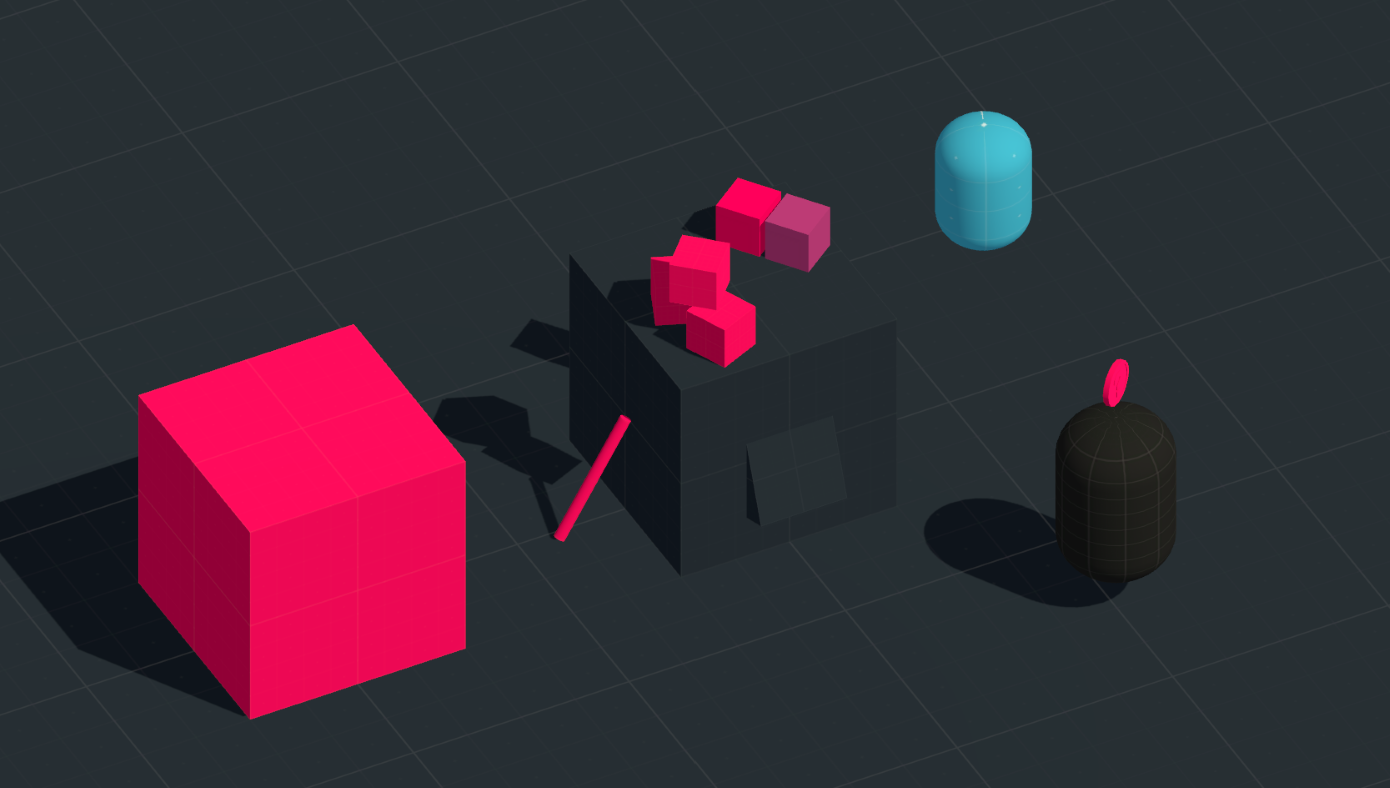
\includegraphics[width=1.0\textwidth]{Environments/devWorld.png}
\caption{An image of the Dev World.}
\label{fig:devWorld}
\end{figure}

\subsection{Touchy Island}
\label{subsec:touchyIsland}
Whereas the Dev World was created and developed along with the prototypes, Touchy Island was created specifically for use during the user evaluations. Touchy Island is like a small playground or game-like experience, where the player can interact with a couple of different types of creatures and objects on a small floating island. The main idea is that the creatures all have moods and their moods are affected by their surroundings. Each of these creatures also have their own small quirks or features, which differentiate them from the other types and was meant to encourage the players to interact with them in certain ways without the need for complicated instructions\footnote{As part of the planning for the development of Touchy Island we prepared a design document. It contains descriptions of several of the elements that went into the final version of the sandbox, although it wasn't kept completely up to date throughout the process. The design document can be found in Appendix \ref{apx:touchyIslandDesignDocument}.}. The four creature types present on the island are the Rock creatures, the Cherry creatures, the Mole creatures and the Cloud creatures.

The Rock creatures start out as small and almost cube shaped. Their shape allows them to be stacked on top of each other, if that's what the player would like to do. The player can then try to move around stacks of Rock creatures while playing a balancing game of sorts. The Rock creatures move around by rolling onto one of the sides it's not currently standing on, like a dice rolling. This also means that they sometimes lie on their sides, their backs or even their faces. The Rock creatures are the only ones that age and grow. Over time the Rock creatures grow old and when this happens, they will be enveloped in a cloud of smoke and they will emerge larger and with crystal hair and a mustache. Rock creatures are also the only creatures that die of old age.

\begin{figure}[h]
\centering
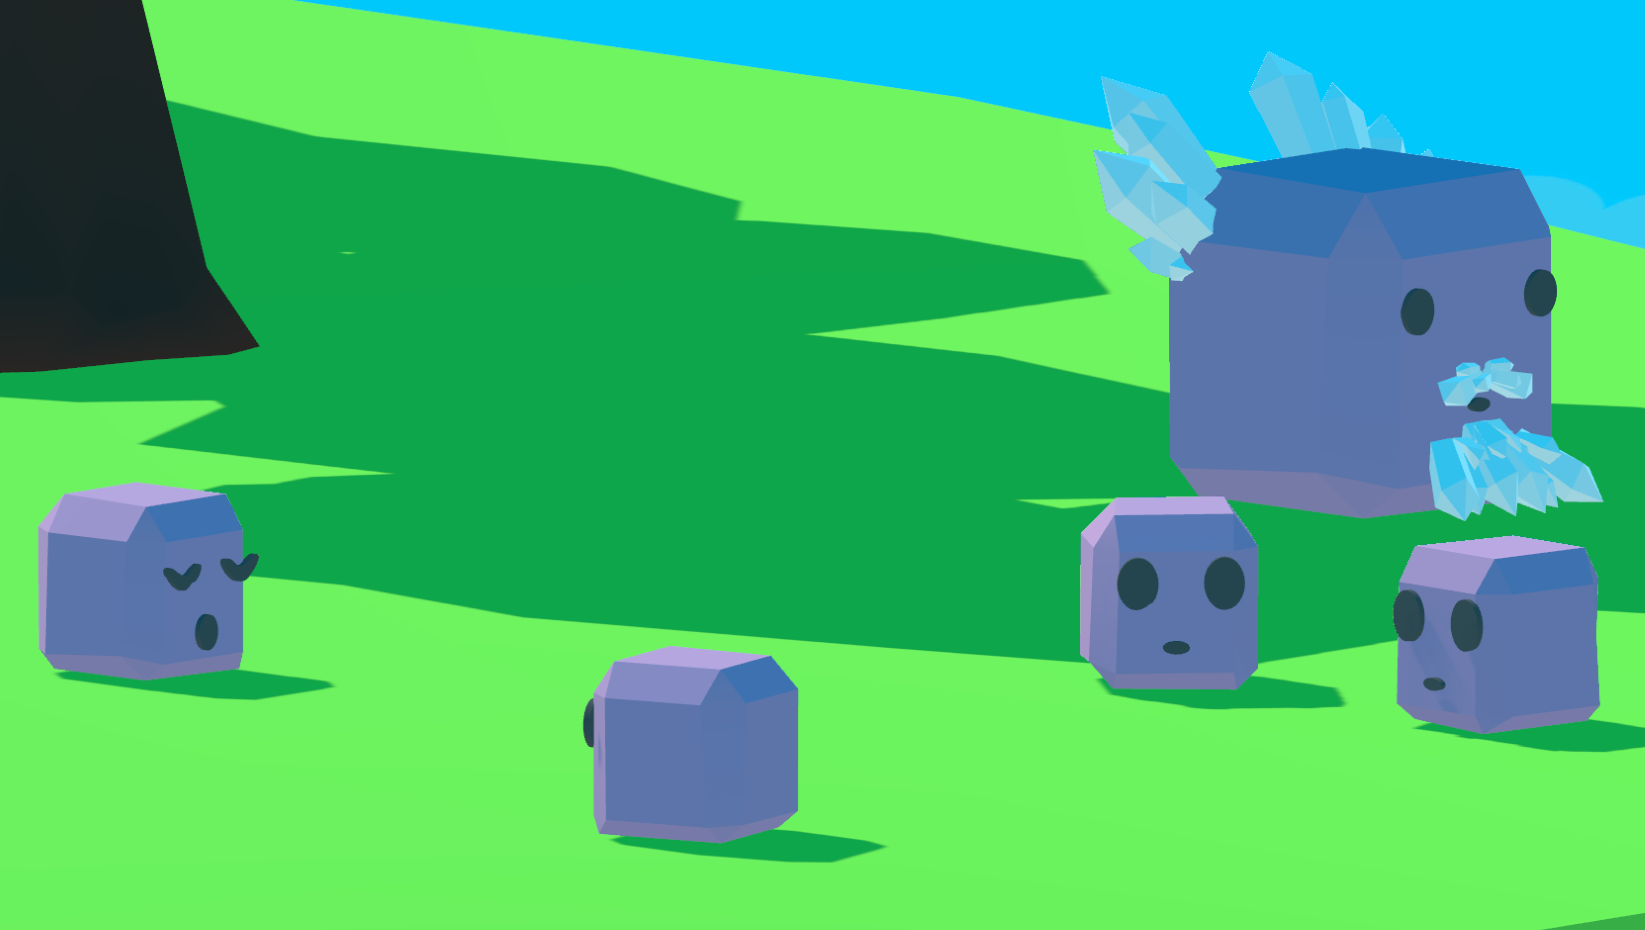
\includegraphics[height=6cm]{Environments/rockCreatures.png}
\caption{An image of the Rock creatures.}
\label{fig:rockCreatures}
\end{figure}

The Cherry creatures start their lives growing from the cherry trees. When they are mature, they drop to the ground and start roaming their environment. They move by jumping around, which also makes them hard to catch, when they are not resting for a while. The size of the Cherry creatures makes them more manageable in terms of their size compared to the other larger creatures. Originally we wanted the Cherry creatures to come in pairs connected by their stem and a joint so that they could be pulled apart, but we opted to let the bamboo, mentioned below, serve that purpose instead.

\begin{figure}[h]
\centering
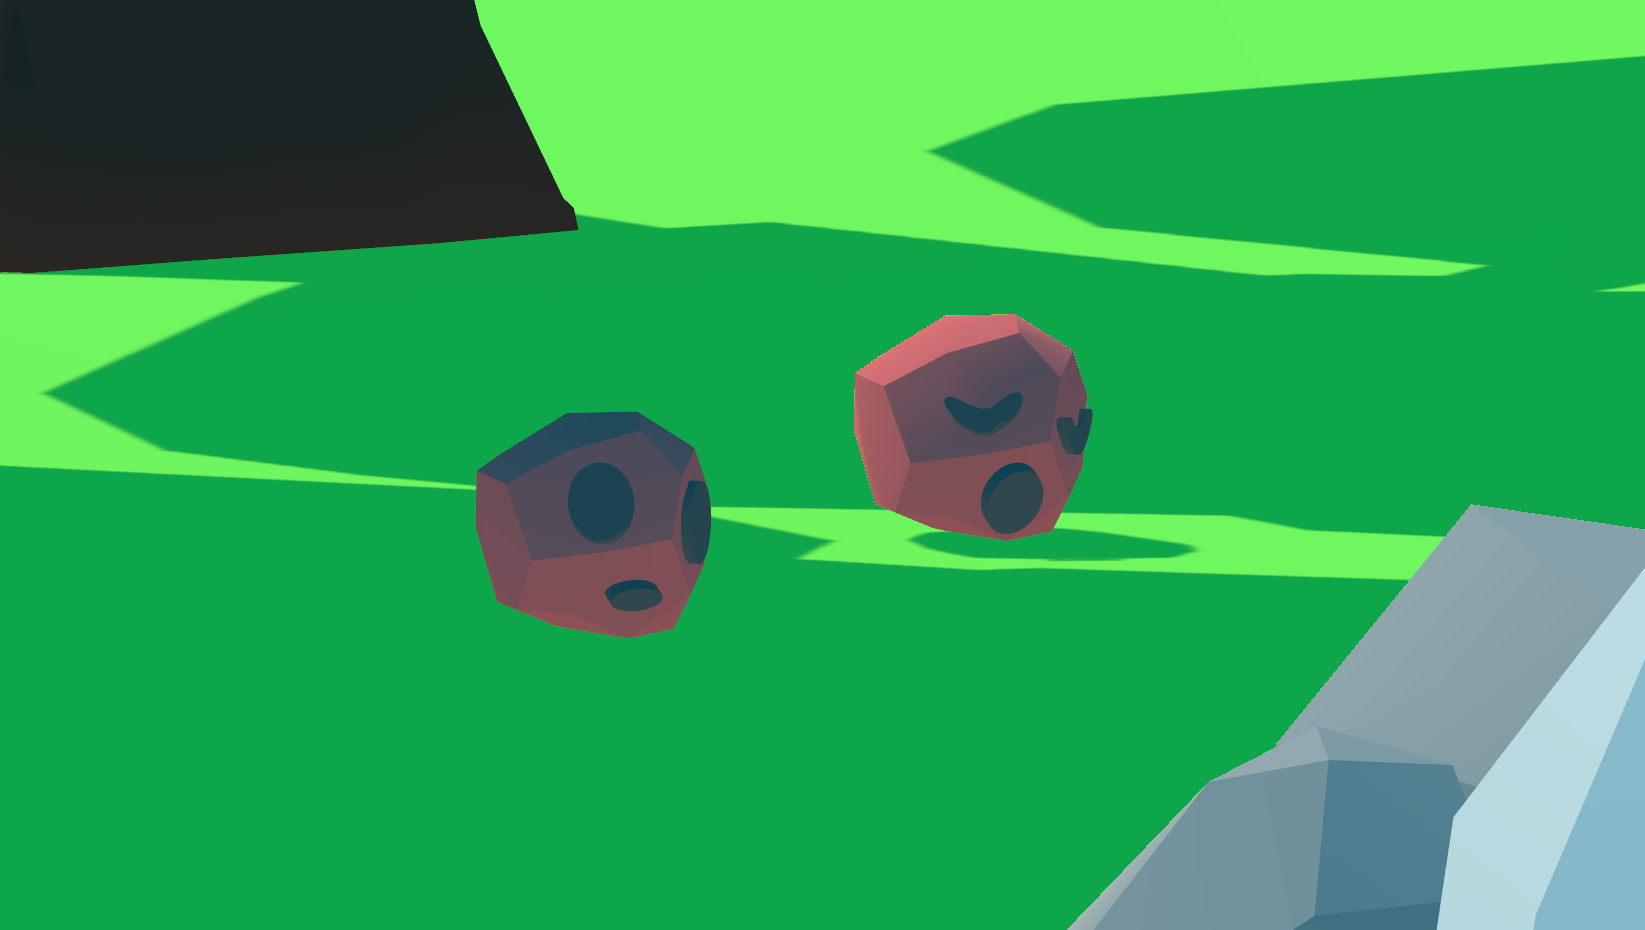
\includegraphics[height=6cm]{Environments/cherryCreatures.png}
\caption{An image of the Cherry creatures.}
\label{fig:cherryCreatures}
\end{figure}

The Mole creatures are capsule shaped creatures that stick their heads out of holes. When touched or hit, they bounce up and down in a spring-like fashion, usually drawing players to hit them even more. When hit hard they even jump out of their holes completely. When grouped together, they could be compared to a game of whack-a-mole.  They only move in a straight line up and down, but can also spin around. The Mole creatures are the only ones that don't have an interaction, when the player tries to grab them using the trigger button.

\begin{figure}[h]
\centering
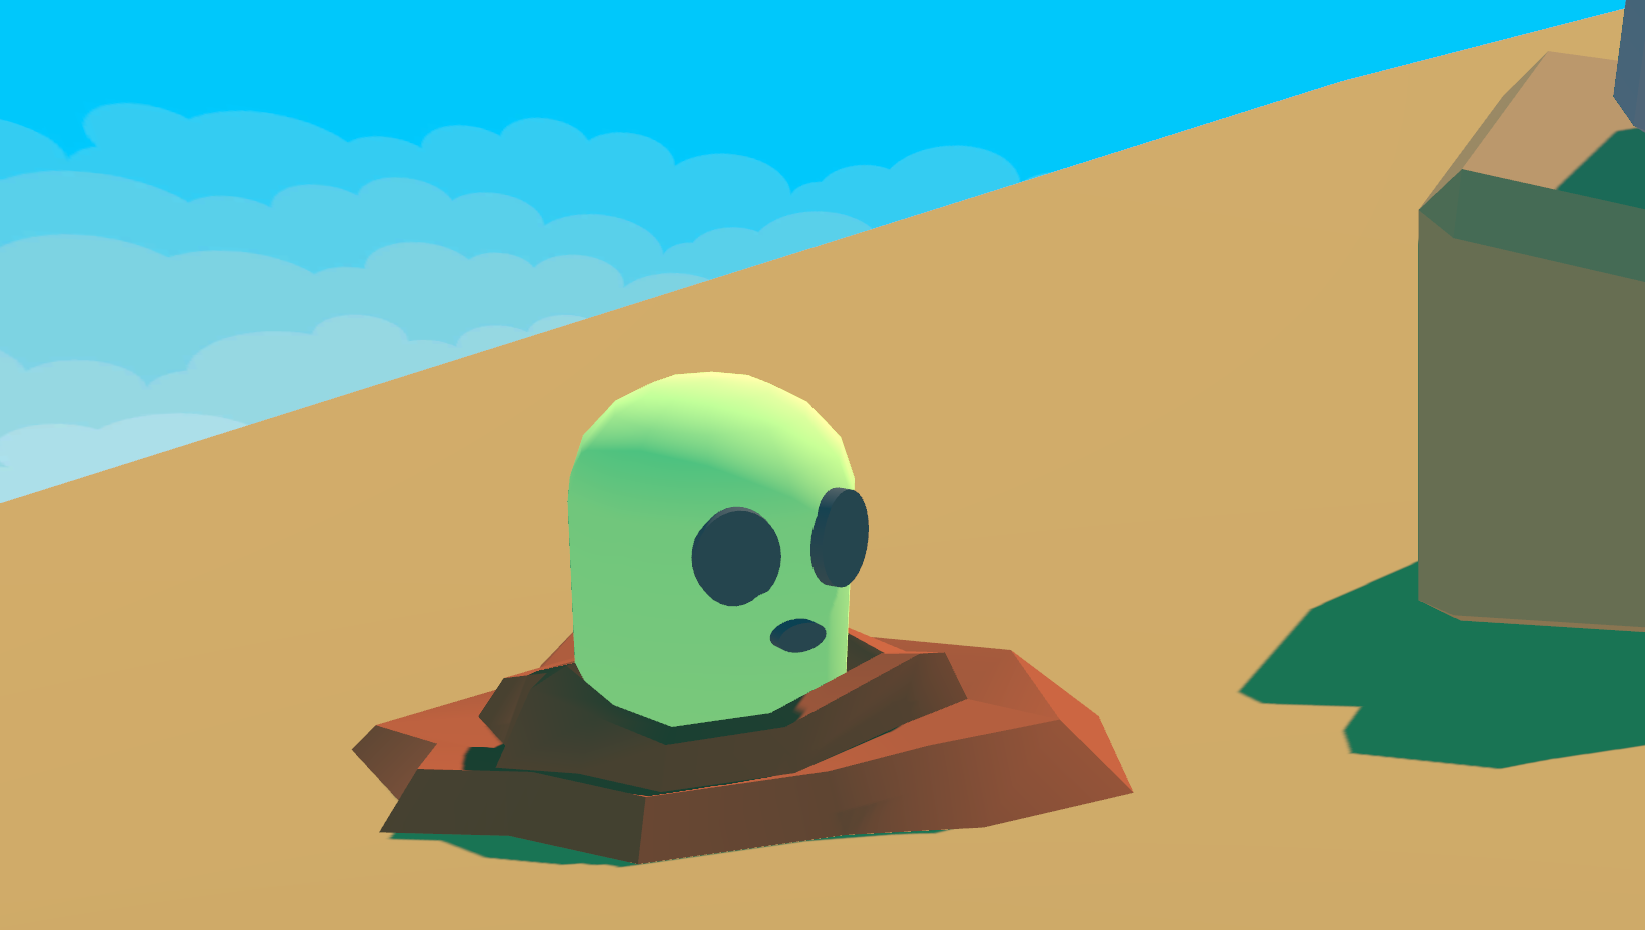
\includegraphics[height=6cm]{Environments/moleCreatures.png}
\caption{An image of the Mole creatures.}
\label{fig:moleCreatures}
\end{figure}

The Cloud creatures float around on each of their spot around the island. They can be pushed around if done gently, but will always try to find a comfortable hovering height over the ground. The Cloud creatures are extremely delicate and can't handle hard hits or grabs. If the player chooses to grab or hit a cloud creature they are killed and vanish in a cloud of smoke. So in order for the player to interact with the cloud creature they need to employ a gentle touch. This encourages the players to handle the Cloud creatures differently from Rock and Cherry creatures that can be grabbed, although that difference can both result in the gentle care of the Cloud creatures or their demise as players try grabbing or hitting them all.

\begin{figure}[h]
\centering
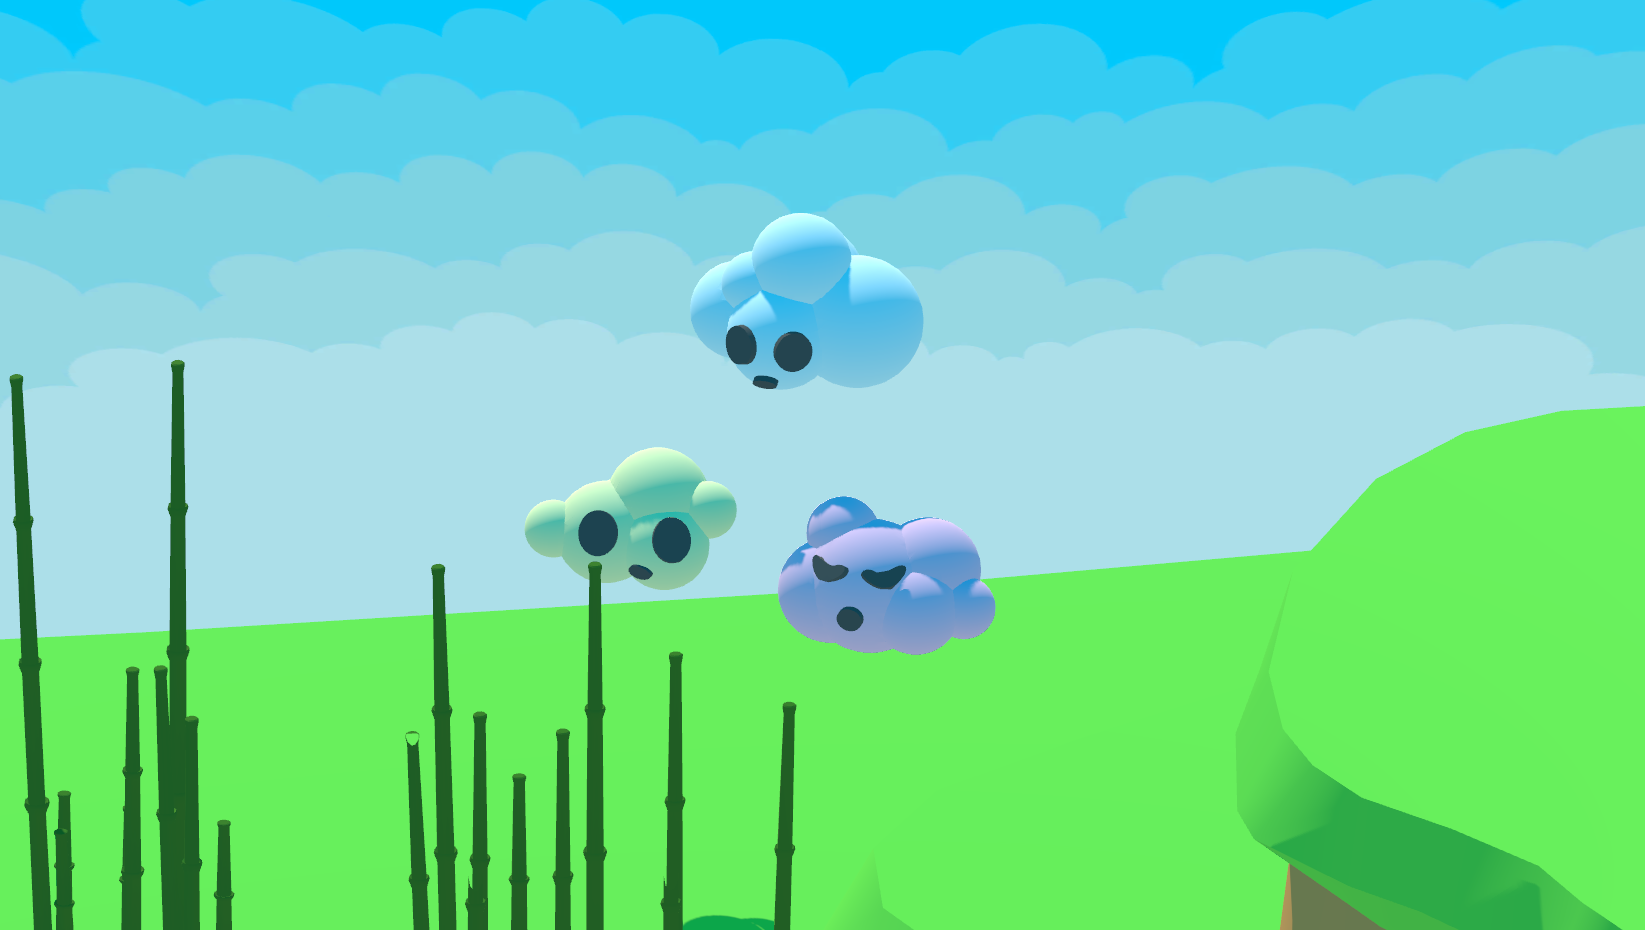
\includegraphics[height=6cm]{Environments/cloudCreatures.png}
\caption{An image of the Cloud creatures.}
\label{fig:cloudCreatures}
\end{figure}

The creatures all have moods which are affected by their surroundings. Creatures can be in one of four different moods: Neutral, Happy, Sad and Angry. Besides allowing moods to increase or decrease over time, the main factor which can change a creature's mood is the player's actions. If a player is gentle and strokes or pets a creature they will become increasingly happy, up till a point where they might even start singing which can make other nearby creatures happier. On the other hand, if the player is throwing or hitting a creature it will become sadder and angrier and surrounding creatures will become sad. The easiest way to make creatures sad is to throw one of their friends over the edge of the island or to poof a cloud by hitting or grabbing it, resulting in their death. A creature's current mood is displayed by their facial expression and by sound effects. Creatures all have a face which can look neutral, happy, sad or angry. Along with that, they also have temporary facial expressions which display the effect of an action. When petted for a while a creature's eyes will turn into hearts, for instance. This way the creatures give the player feedback on the effect of their actions.

As mentioned above there are also two interactive objects besides the creatures. They both exist to allow the player to experience different interactions. The interactive objects are bamboos and movable rocks. On the island there is a small bamboo forest. If the player so desires, they can break off the bamboo from its root and use it as a stick to throw, push or hit things with. The bamboos are connected to their roots using joints which have a certain break force. This allows the player to be able to grab the bamboo and then pull it off its root, but they can also be hit to break them. The movable rocks are essentially just rocks that are scattered around the island but aren't stuck in the ground. We disabled the grabbing feature from the rocks and made them rather heavy so that players could experience the different feel of weight when pushing and lifting the rocks with the different hands. Finally, the island also has static objects like small crystals, immovable rocks, the cherry trees and some plateaus. When the player interacts with these they'll really see the position filtering in action for the Physics Hand along with the real hand visualization and notice the fact that our implementation of the Job Simulator Hand moves straight through such objects. 

\begin{figure}[h]
\centering
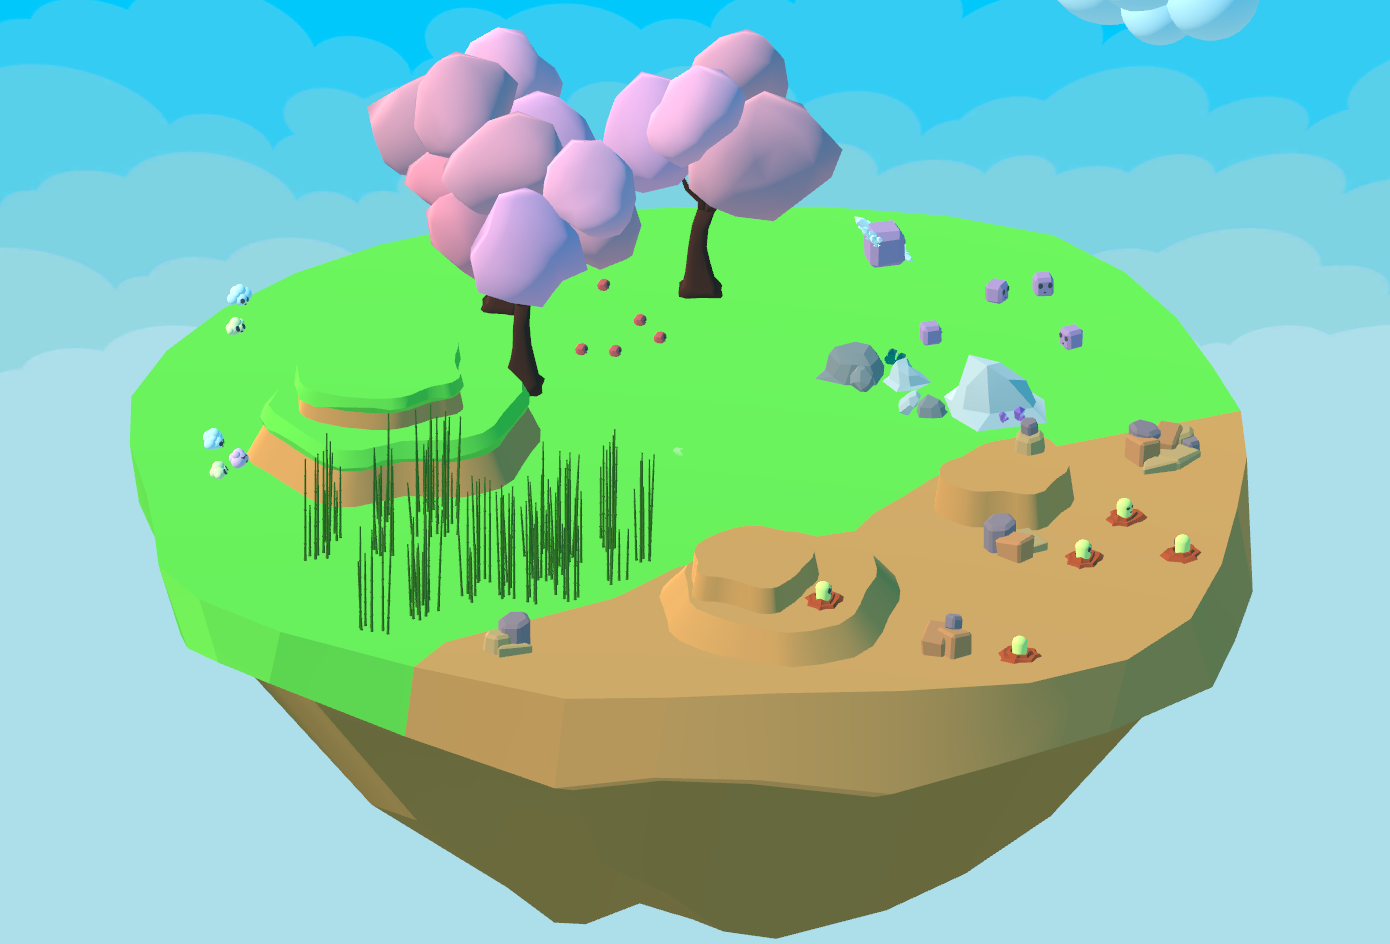
\includegraphics[height=10cm]{Environments/touchyIsland.png}
\caption{An image of Touchy Island.}
\label{fig:touchyIsland}
\end{figure}

These different creatures and objects all have their distinct purpose in the world because of their unique features. These are not implemented to have diversity, but to draw in the player and make them want to interact with the environment. The reason for the creatures to have moods that are affected by the player's actions is to make the players want to interact with them and thereby use the hands. This also leads back into the decision to make a more game-like experience rather than making another environment like the Dev World or no new environment at all. By first guiding testers through through a set of interactions in the Dev World and learn the features of the hand, releasing them into this playful sandbox would be a different experience which is closer to the context in which the hands would be used commercially. Since the Dev World is a guided, more abstract environment without distractions and Touchy Island is a more free-form contextualized experience they complement each other and combined give us better results than if we had tested in only one of these environments.
